\begin{anexosenv}

\partanexos

\chapter{Gráficos de Filtragem}

As figuras abaixo são representações de sinais no domínio do tempo, seguidas de sinais no domínio da frequência. Utilizou-se duas janelas de dois segundos de cada música para realizar as representações. 

Cada representação conta com uma filtragem em uma determinada frequência de corte, de forma que se consiga visualizar a modificação do sinal conforme a aplicação dos filtros. As Figuras \ref{fig24} a \ref{fig31} se referem a uma música, enquanto as Figuras \ref{fig32} a \ref{fig39} correspondem a outra música utilizada na prova de conceito.
 
\begin{figure}[h]
	\centering
    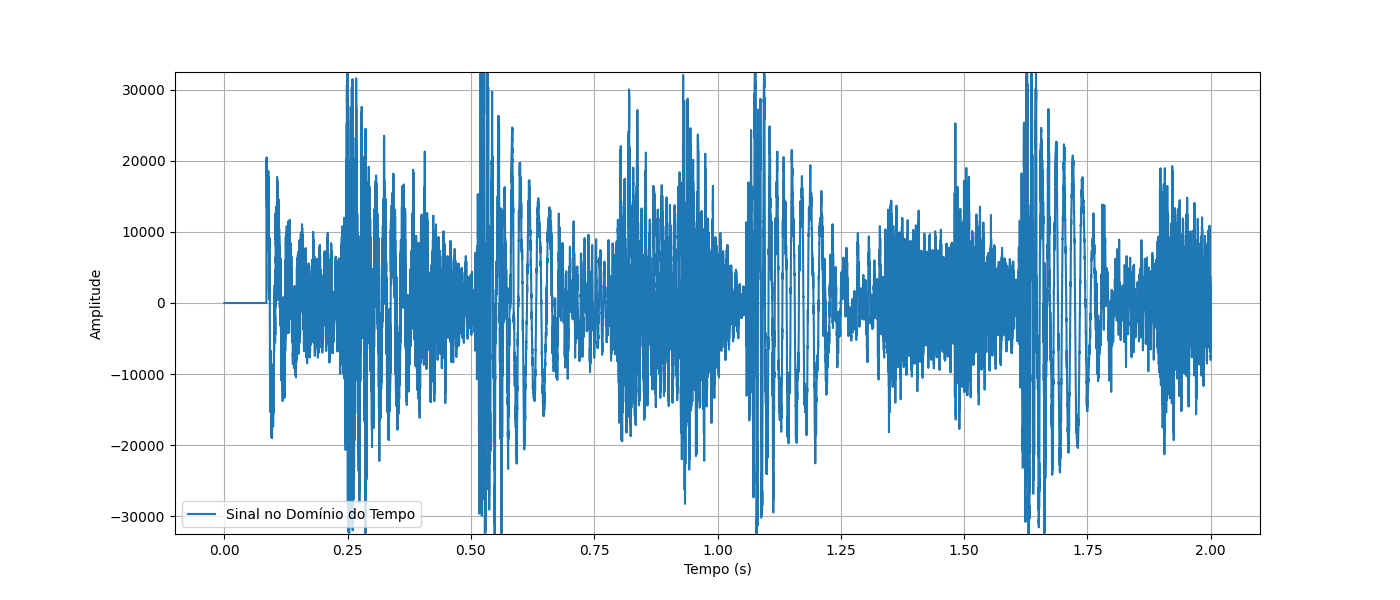
\includegraphics[width=\textwidth]{figuras/fig24.png}
	\caption{música 1 no domínio do tempo com uma $f_c$ de 20 Hz}
	\label{fig24}
\end{figure}

\begin{figure}[h]
	\centering
    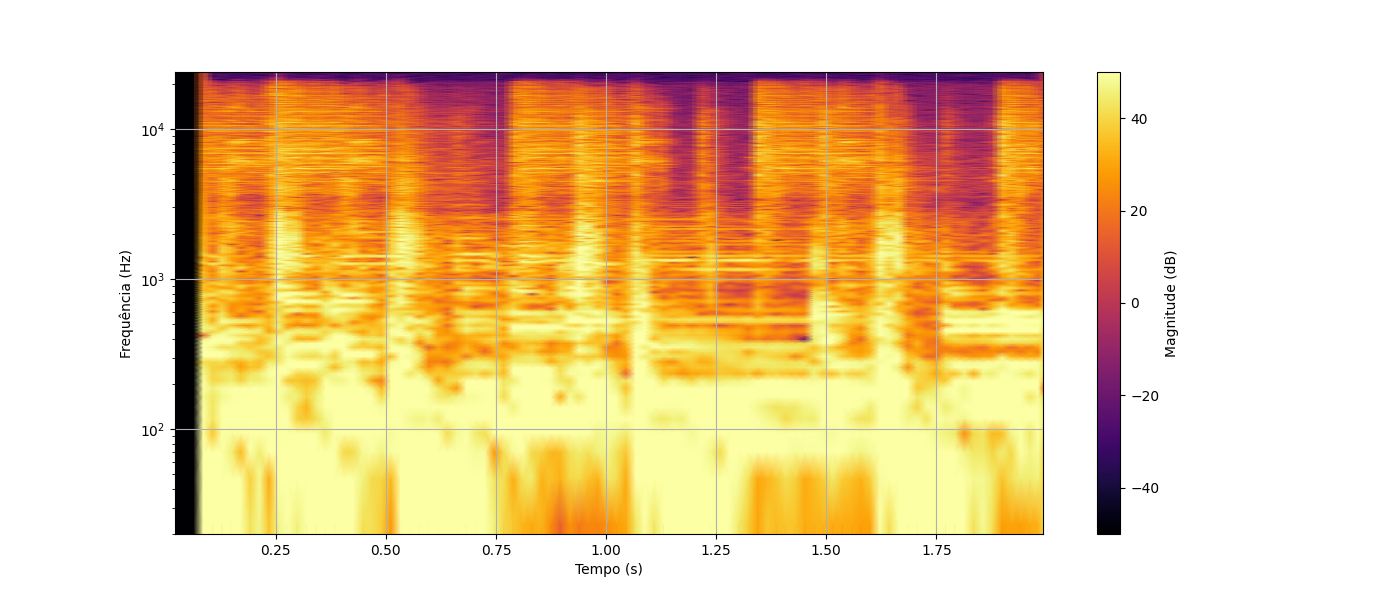
\includegraphics[width=\textwidth]{figuras/fig25.png}
	\caption{música 1 no domínio da frequência com uma $f_c$ de 20 Hz}
	\label{fig25}
\end{figure}

\begin{figure}[h]
	\centering
    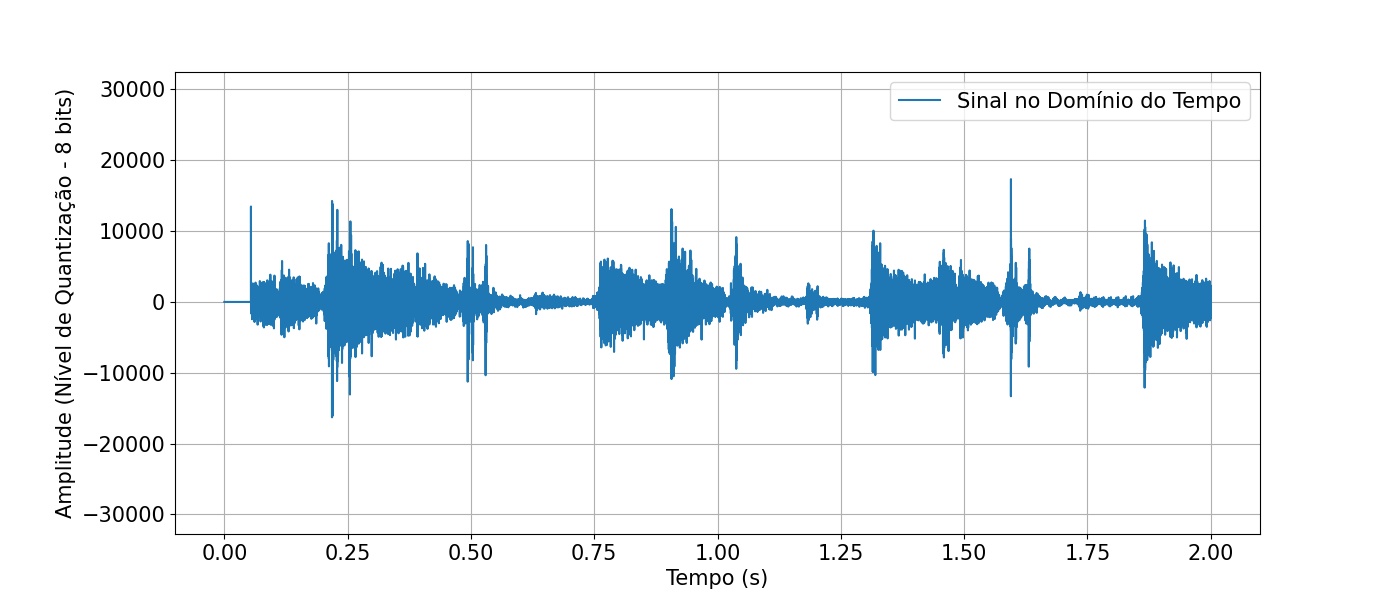
\includegraphics[width=\textwidth]{figuras/fig26.png}
	\caption{música 1 no domínio do tempo com uma $f_c$ de 300 Hz}
	\label{fig26}
\end{figure}

\begin{figure}[h]
	\centering
    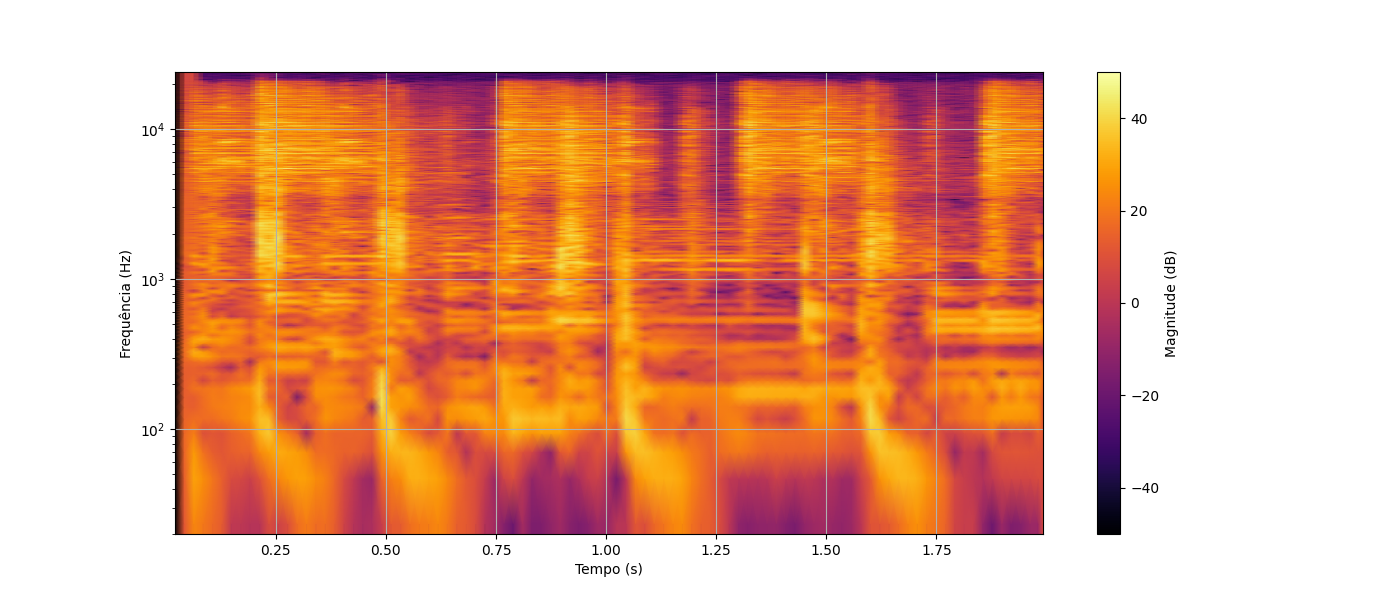
\includegraphics[width=\textwidth]{figuras/fig27.png}
	\caption{música 1 no domínio da frequência com uma $f_c$ de 300 Hz}
	\label{fig27}
\end{figure}

\begin{figure}[h]
	\centering
    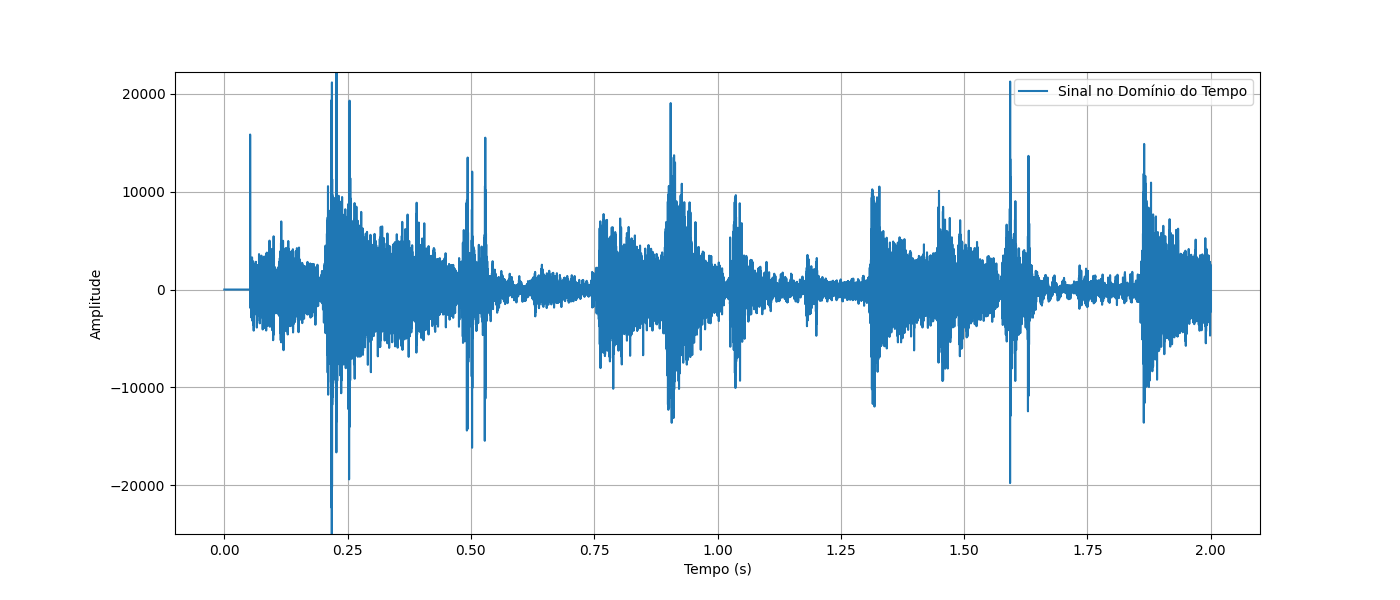
\includegraphics[width=\textwidth]{figuras/fig28.png}
	\caption{música 1 no domínio do tempo com uma $f_c$ de 4 kHz}
	\label{fig28}
\end{figure}

\begin{figure}[h]
	\centering
    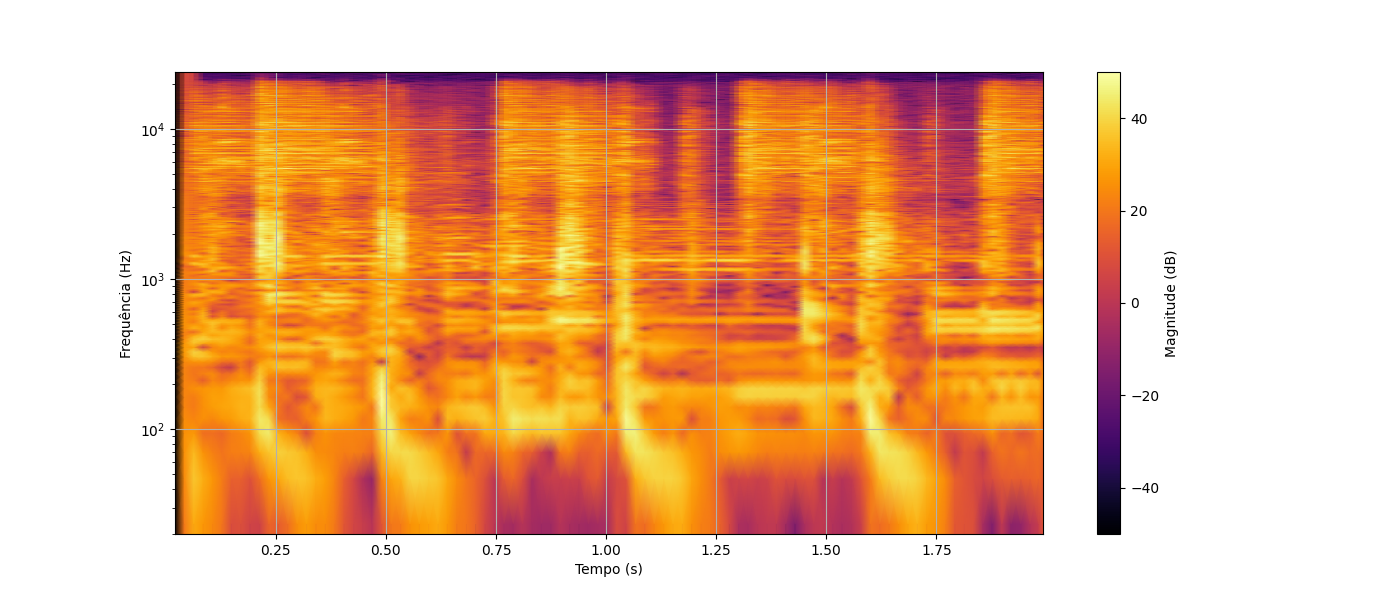
\includegraphics[width=\textwidth]{figuras/fig29.png}
	\caption{música 1 no domínio da frequência com uma $f_c$ de 4 kHz}
	\label{fig29}
\end{figure}

\begin{figure}[h]
	\centering
    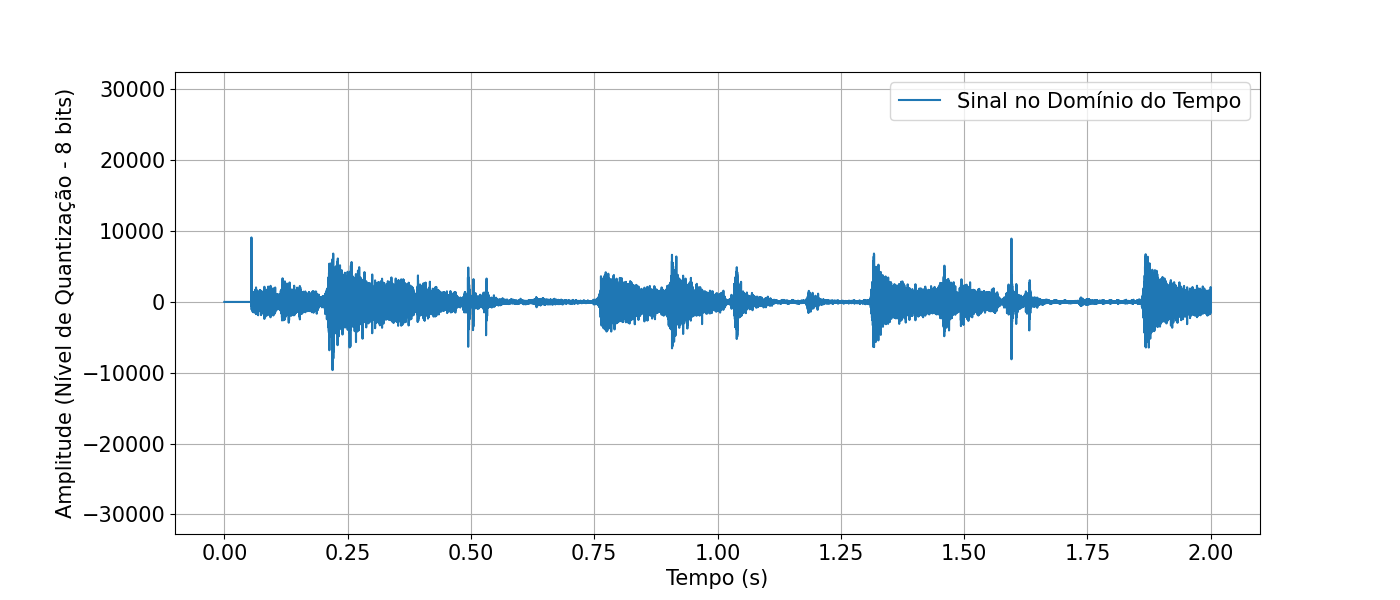
\includegraphics[width=\textwidth]{figuras/fig30.png}
	\caption{música 1 no domínio do tempo com uma $f_c$ de 24 kHz}
	\label{fig30}
\end{figure}

\begin{figure}[h]
	\centering
    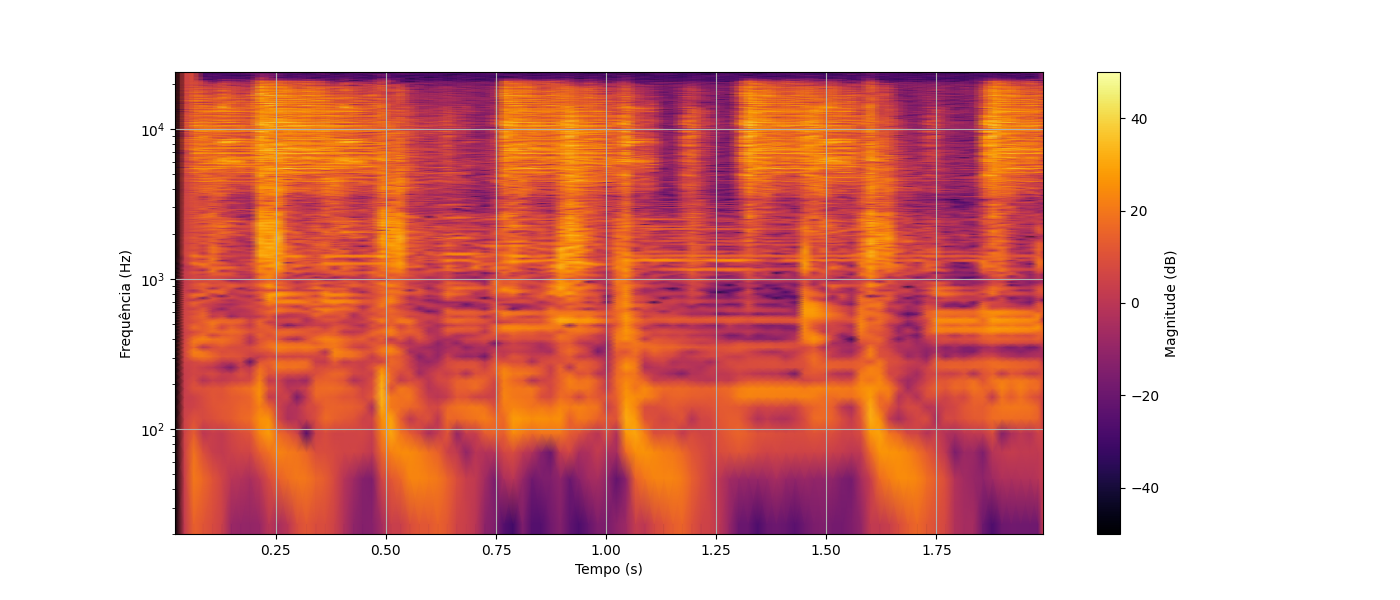
\includegraphics[width=\textwidth]{figuras/fig31.png}
	\caption{música 1 no domínio da frequência com uma $f_c$ de 24 kHz}
	\label{fig31}
\end{figure}

\begin{figure}[h]
	\centering
    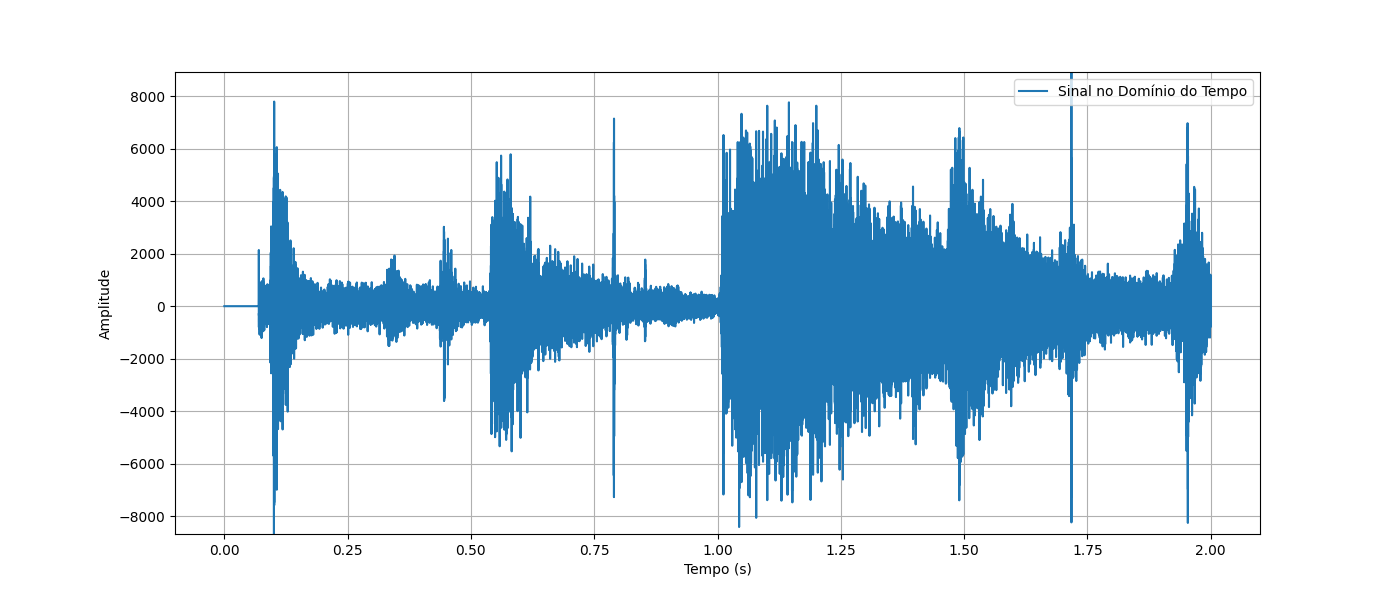
\includegraphics[width=\textwidth]{figuras/fig32.png}
	\caption{música 2 no domínio do tempo com uma $f_c$ de 24 kHz}
	\label{fig32}
\end{figure}

\begin{figure}[h]
	\centering
    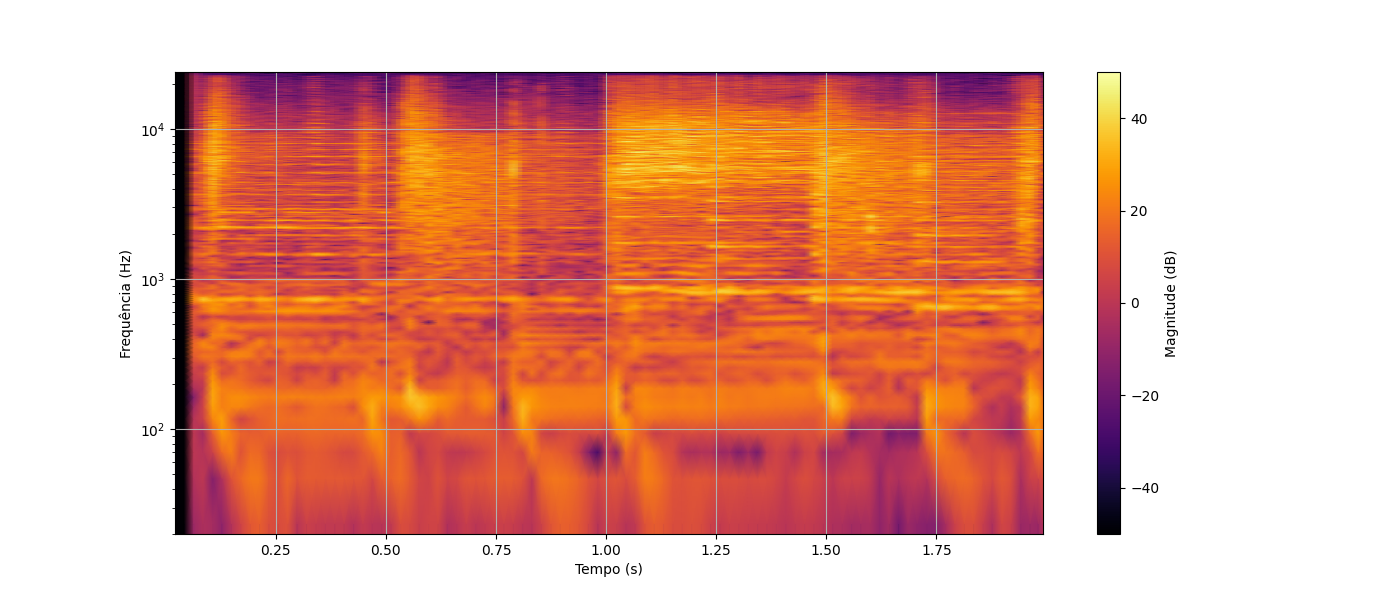
\includegraphics[width=\textwidth]{figuras/fig33.png}
	\caption{música 2 no domínio da frequência com uma $f_c$ de 24 kHz}
	\label{fig33}
\end{figure}

\begin{figure}[h]
	\centering
    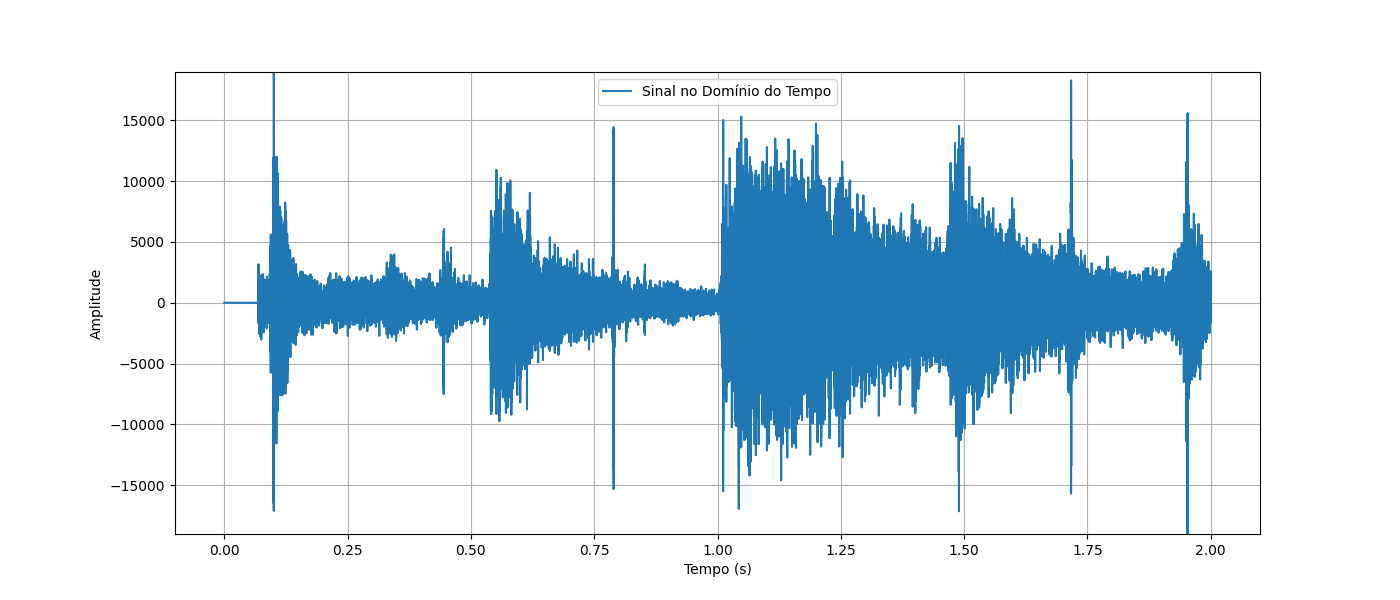
\includegraphics[width=\textwidth]{figuras/fig34.png}
	\caption{música 2 no domínio do tempo com uma $f_c$ de 4 kHz}
	\label{fig34}
\end{figure}

\begin{figure}[h]
	\centering
    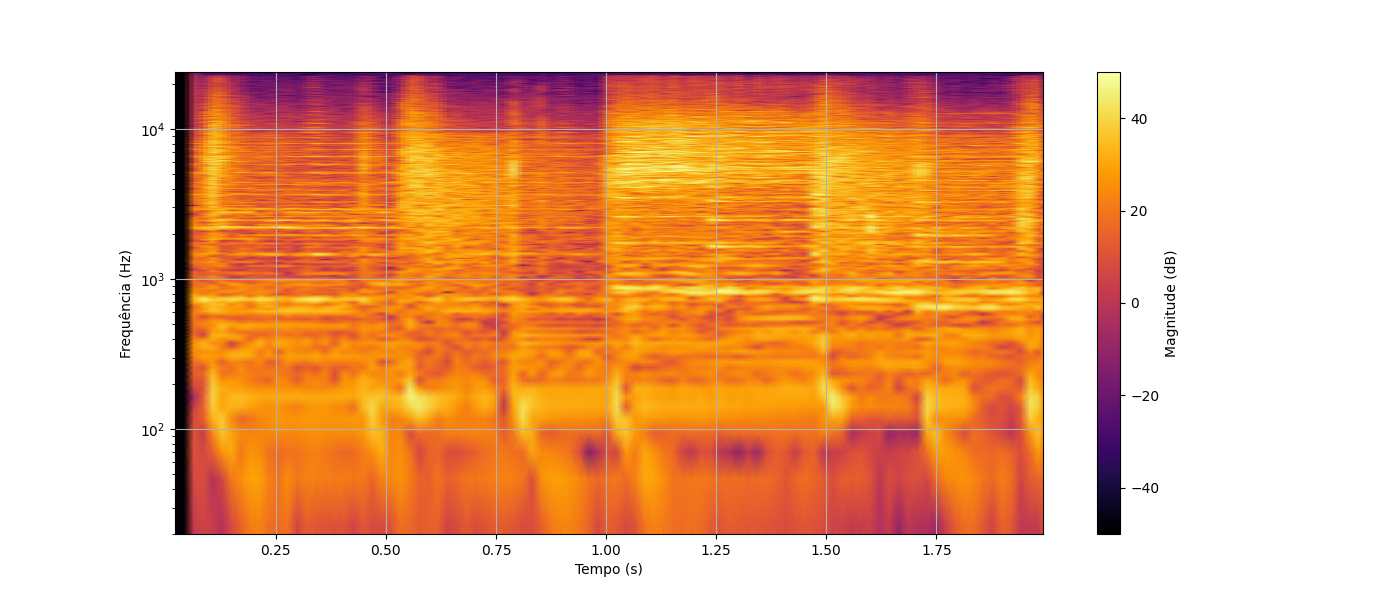
\includegraphics[width=\textwidth]{figuras/fig35.png}
	\caption{música 2 no domínio da frequência com uma $f_c$ de 4 kHz}
	\label{fig35}
\end{figure}

\begin{figure}[h]
	\centering
    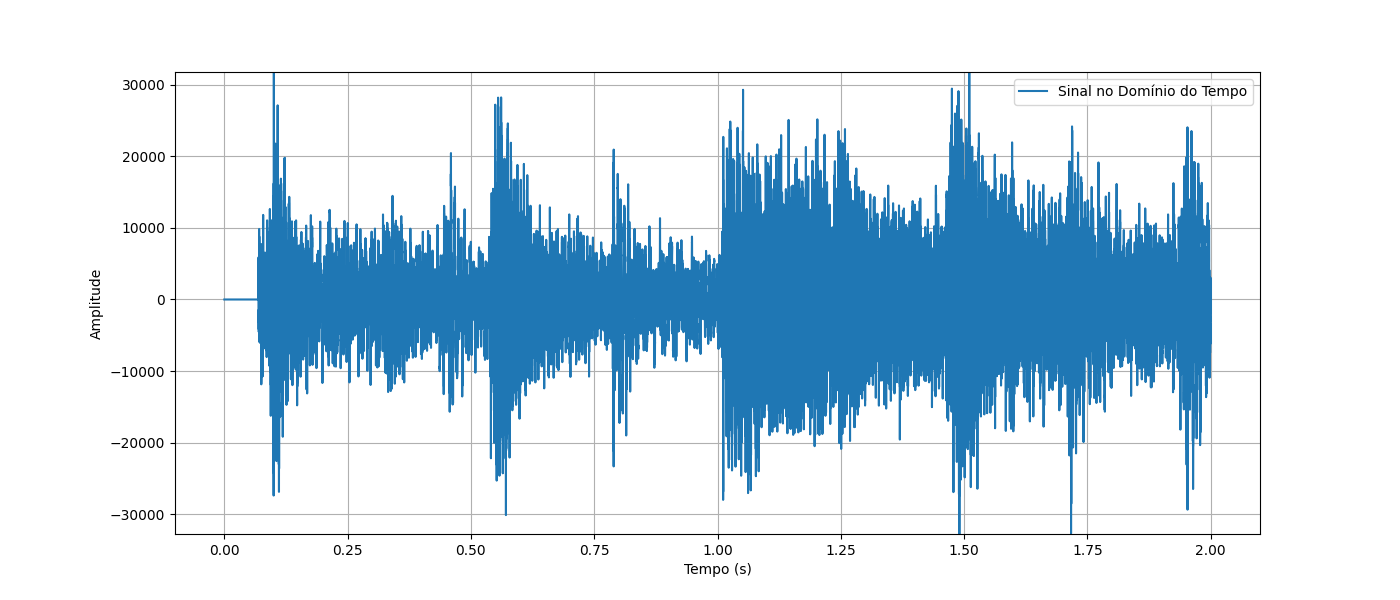
\includegraphics[width=\textwidth]{figuras/fig36.png}
	\caption{música 2 no domínio do tempo com uma $f_c$ de 300 Hz}
	\label{fig36}
\end{figure}

\begin{figure}[h]
	\centering
    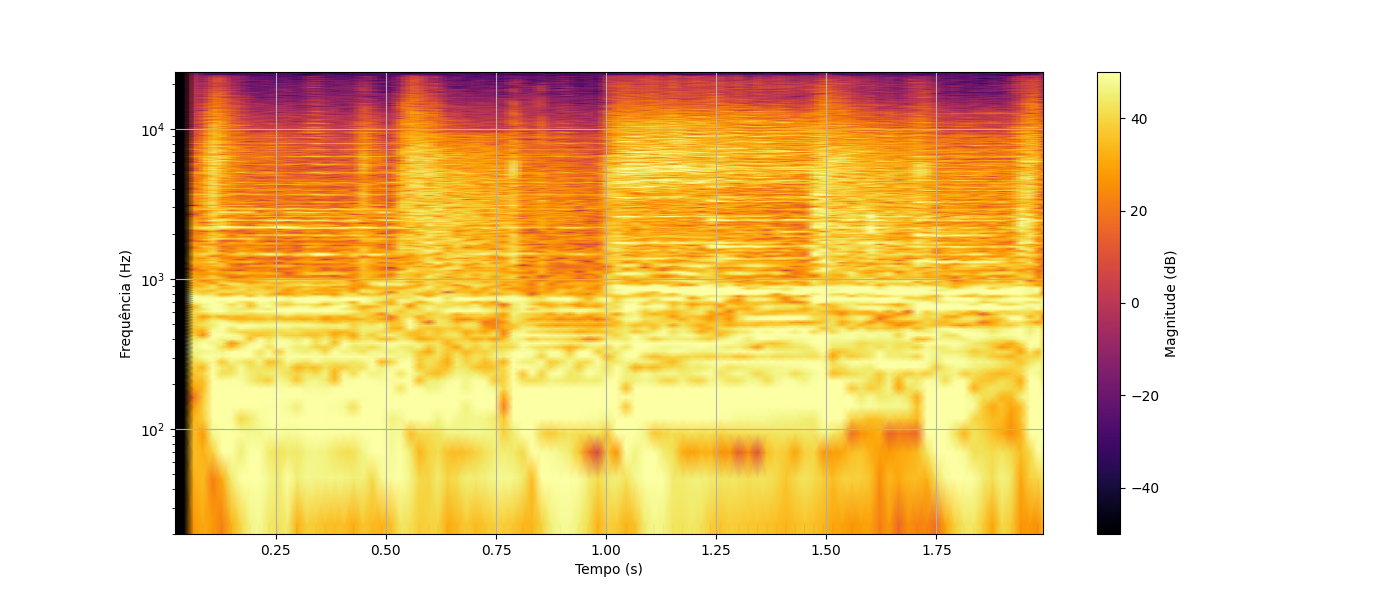
\includegraphics[width=\textwidth]{figuras/fig37.png}
	\caption{música 2 no domínio da frequência com uma $f_c$ de 300 Hz}
	\label{fig37}
\end{figure}

\begin{figure}[h]
	\centering
    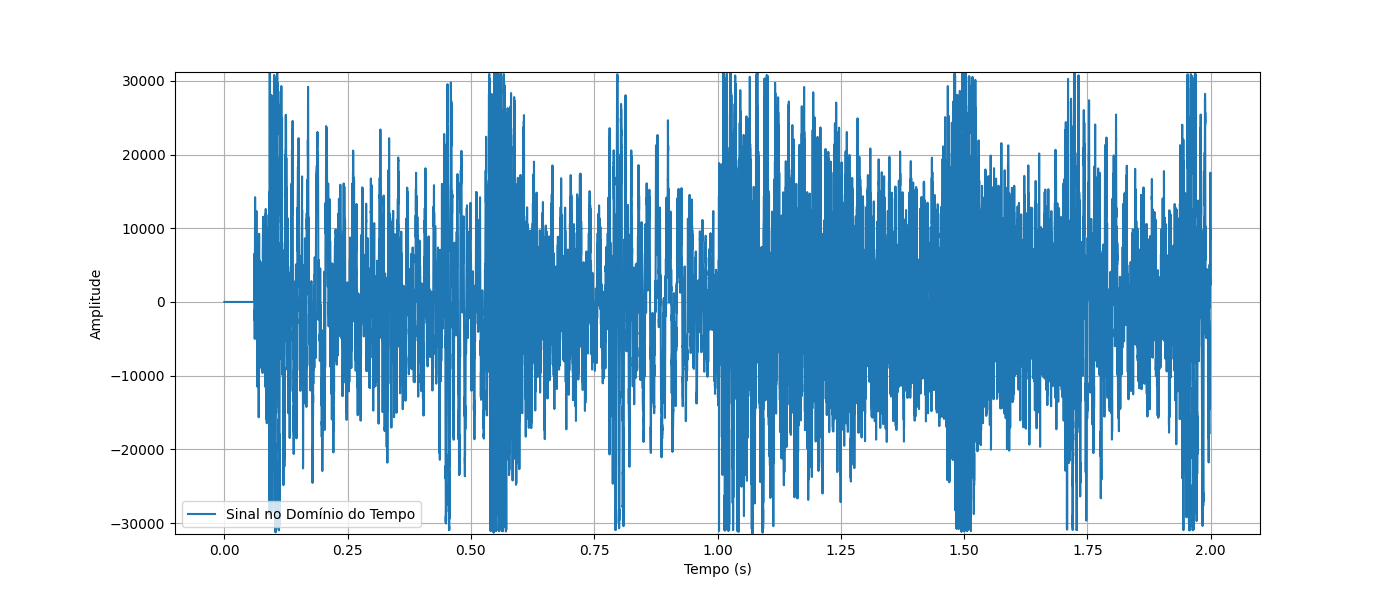
\includegraphics[width=\textwidth]{figuras/fig38.png}
	\caption{música 2 no domínio do tempo com uma $f_c$ de 20 Hz}
	\label{fig38}
\end{figure}

\begin{figure}[h]
	\centering
    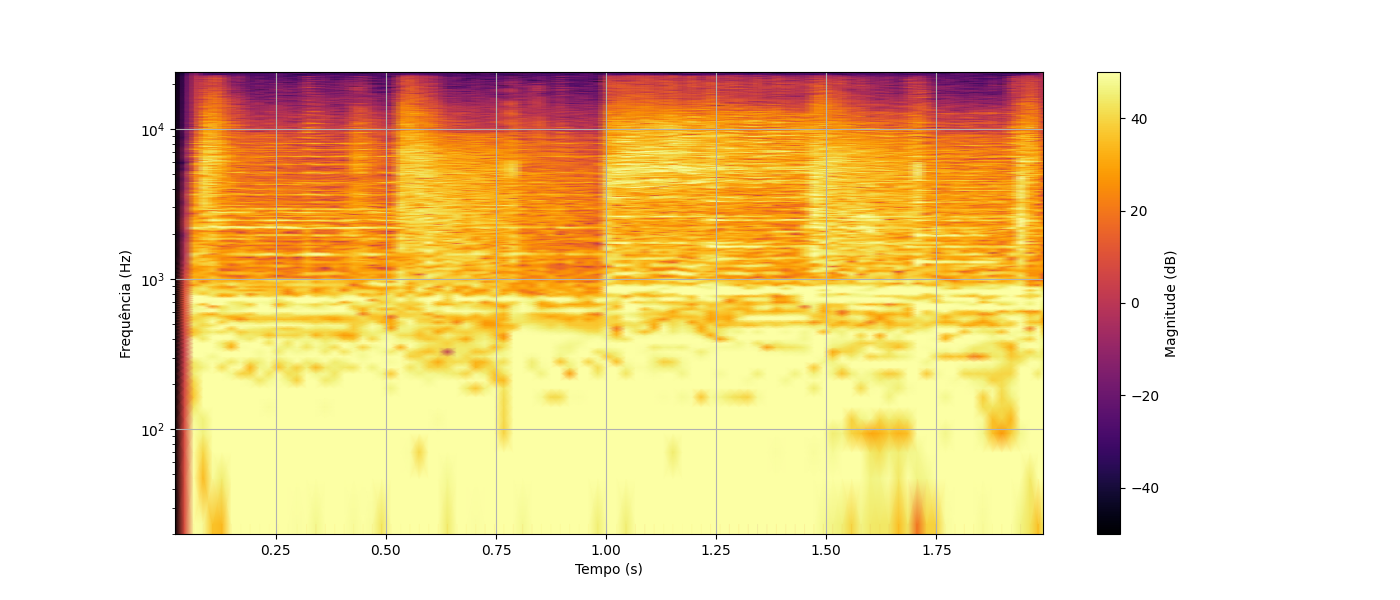
\includegraphics[width=\textwidth]{figuras/fig39.png}
	\caption{música 2 no domínio da frequência com uma $f_c$ de 20 Hz}
	\label{fig39}
\end{figure}

\end{anexosenv}